\chapter{Квадраттық түбір алгоритмдер}

\index{квадраттық түбір алгоритм}

\key{Квадраттық түбір алгоритмі} -- уақытша күрделілігінде
квадрат түбірі бар алгоритм.  $O(\sqrt n)$ күрделілігі $O(n)$-нен
тез болғанымен, $O(\log n)$-нен баяу болуына байланысты оны ''кемшілікті логарифм'' 
ретінде де қарастыруға болады. Қандай жағдай болмасын көптеген түбір алгоритмдер қолданыста жылдам, ыңғайлы және тиімді болып келеді. 

Мысалға төмендегі есепті қарастырайық:
берілген позициядағы элементті өзгерту және
берілген аралық бойынша қосындыны есептеу
операцияларын қолдайтын деректер құрылымын құруымыз керек.
Осыған дейін біз бұл есепті
екі операцияны $O(\log n)$ уақытта қолдайтын
бинарлы индекстелген дарақ немесе кесінділер дарағы 
арқылы шығарған едік. Ал енді $O(1)$ уақытта
элементтерді өзгертуге және $O(\sqrt n)$ уақытта 
қосындыларды есептеуге мүмкіндік беретін квадраттық 
түбір құрылымын пайдаланып, басқа жолмен шешеміз.

Идеясы жиымды өлшемі $\sqrt n$ болатын \emph{блоктар}ға бөлу
және әр блок үшін ішіндегі элементтер қосындысын сақтауға негізделеді.
Мысалы, 16 элементтен тұратын жиым төмендегідей 4 элементтік блоктарға бөлінеді:

\begin{center}
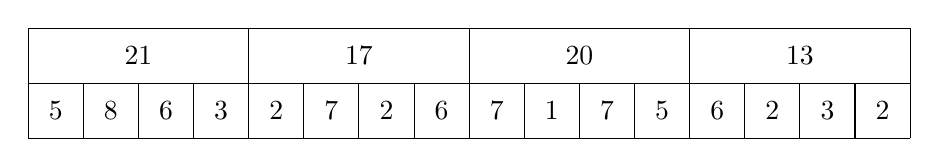
\begin{tikzpicture}[scale=0.7]
\draw (0,0) grid (16,1);

\draw (0,1) rectangle (4,2);
\draw (4,1) rectangle (8,2);
\draw (8,1) rectangle (12,2);
\draw (12,1) rectangle (16,2);

\node at (0.5, 0.5) {5};
\node at (1.5, 0.5) {8};
\node at (2.5, 0.5) {6};
\node at (3.5, 0.5) {3};
\node at (4.5, 0.5) {2};
\node at (5.5, 0.5) {7};
\node at (6.5, 0.5) {2};
\node at (7.5, 0.5) {6};
\node at (8.5, 0.5) {7};
\node at (9.5, 0.5) {1};
\node at (10.5, 0.5) {7};
\node at (11.5, 0.5) {5};
\node at (12.5, 0.5) {6};
\node at (13.5, 0.5) {2};
\node at (14.5, 0.5) {3};
\node at (15.5, 0.5) {2};

\node at (2, 1.5) {21};
\node at (6, 1.5) {17};
\node at (10, 1.5) {20};
\node at (14, 1.5) {13};

\end{tikzpicture}
\end{center}

Аталған құрылымда жиым элементтерін өзгерту 
жеңіл. Өйткені әр жаңартудан кейін 1 ғана блоктың
қосындысы өзгереді, ал ол өз кезегінде $O(1)$
уақытта орындалады. Мысалы, төмендегі суретте
элементтің мәні және оған сәйкес блок қалай
өзгеретіні көрсетілген:

\begin{center}
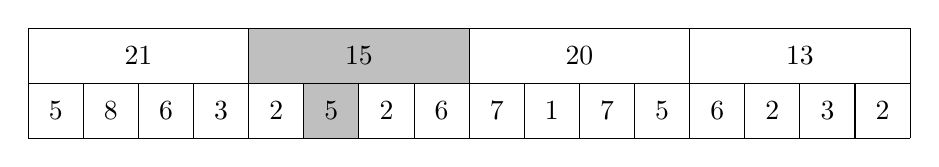
\begin{tikzpicture}[scale=0.7]
\fill[color=lightgray] (5,0) rectangle (6,1);
\draw (0,0) grid (16,1);

\fill[color=lightgray] (4,1) rectangle (8,2);
\draw (0,1) rectangle (4,2);
\draw (4,1) rectangle (8,2);
\draw (8,1) rectangle (12,2);
\draw (12,1) rectangle (16,2);

\node at (0.5, 0.5) {5};
\node at (1.5, 0.5) {8};
\node at (2.5, 0.5) {6};
\node at (3.5, 0.5) {3};
\node at (4.5, 0.5) {2};
\node at (5.5, 0.5) {5};
\node at (6.5, 0.5) {2};
\node at (7.5, 0.5) {6};
\node at (8.5, 0.5) {7};
\node at (9.5, 0.5) {1};
\node at (10.5, 0.5) {7};
\node at (11.5, 0.5) {5};
\node at (12.5, 0.5) {6};
\node at (13.5, 0.5) {2};
\node at (14.5, 0.5) {3};
\node at (15.5, 0.5) {2};

\node at (2, 1.5) {21};
\node at (6, 1.5) {15};
\node at (10, 1.5) {20};
\node at (14, 1.5) {13};

\end{tikzpicture}
\end{center}

Аралықтағы қосындыны есептеу үшін, дара
элементтер мен олардың арасындағы 
бүтін блоктардан тұратындай етіп, аралықты үшке бөлеміз:

\begin{center}
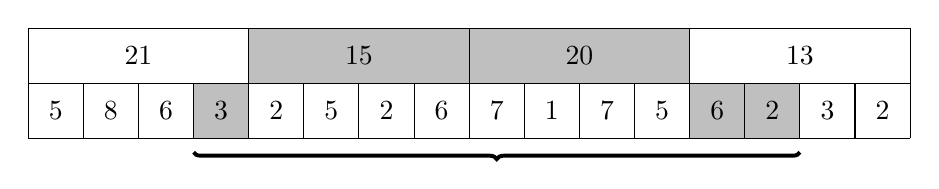
\begin{tikzpicture}[scale=0.7]
\fill[color=lightgray] (3,0) rectangle (4,1);
\fill[color=lightgray] (12,0) rectangle (13,1);
\fill[color=lightgray] (13,0) rectangle (14,1);
\draw (0,0) grid (16,1);

\fill[color=lightgray] (4,1) rectangle (8,2);
\fill[color=lightgray] (8,1) rectangle (12,2);
\draw (0,1) rectangle (4,2);
\draw (4,1) rectangle (8,2);
\draw (8,1) rectangle (12,2);
\draw (12,1) rectangle (16,2);

\node at (0.5, 0.5) {5};
\node at (1.5, 0.5) {8};
\node at (2.5, 0.5) {6};
\node at (3.5, 0.5) {3};
\node at (4.5, 0.5) {2};
\node at (5.5, 0.5) {5};
\node at (6.5, 0.5) {2};
\node at (7.5, 0.5) {6};
\node at (8.5, 0.5) {7};
\node at (9.5, 0.5) {1};
\node at (10.5, 0.5) {7};
\node at (11.5, 0.5) {5};
\node at (12.5, 0.5) {6};
\node at (13.5, 0.5) {2};
\node at (14.5, 0.5) {3};
\node at (15.5, 0.5) {2};

\node at (2, 1.5) {21};
\node at (6, 1.5) {15};
\node at (10, 1.5) {20};
\node at (14, 1.5) {13};

\draw [decoration={brace}, decorate, line width=0.5mm] (14,-0.25) -- (3,-0.25);

\end{tikzpicture}
\end{center}

Дара элементтердің саны да $O(\sqrt n)$,
блоктардың саны да $O(\sqrt n)$ болғандықтан, 
қосынды сұратымы $O(\sqrt n)$ уақыт алады. 
Блоктың өлшемі -- $\sqrt n$, өйткені ол екі затты теңгерімдейді: жиым $\sqrt n$ блоктан, ал әр блок $\sqrt n$ элементтен тұрады. 

Тәжірибеде параметр ретінде дәл $\sqrt n$ мәнін 
қолдану шарт емес, оны $k$ мен $n/k$ арқылы
алмастыра аламыз, мұндағы $k$ $\sqrt n$-ге тең емес. 
Параметр тиімділігі есеп пен енгізуге байланысты.
Мысалы, егер алгоритм блоктарды жиі қарап, 
дара элементтерге сирек жүгінетін болса,
жиымды $k < \sqrt n$ блоктарға, ал әр блокты
$n/k > \sqrt n$ бөлген тиімді.

\section{Алгоритмдерді біріктіру}

Бұл бөлімде біз екі алгоритмді біріктіруге негізделген
екі квадрат түбір алгоритмін талқылаймыз.
Қай жағдайда да алгоритмдердің біреуін ғана қолдана отырып, есепті 
$O(n^2)$ уақытта шығаруға болады. Бірақ, алгоритмдерді біріктіру арқылы
уақытша күрделілігі $O(n \sqrt n)$-ге қысқарады. 

\subsubsection{Жағдайларды қарастыру} % TODO

Бізге $n$ ұяшығы бар екі өлшемдік тор берілген. 
Әр ұяшықта әріп белгіленген. Бізге арақашықтығы ең аз болатын бірдей 
әріпті екі ұяшықты табу тапсырылады. $(x_1,y_1)$ және
$(x_2,y_2)$ ұяшықтарының қашықтығы -- $|x_1-x_2|+|y_1-y_2|$. 
Мысалы, төмендегі торды қарастырайық:

\begin{center}
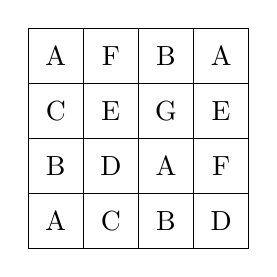
\begin{tikzpicture}[scale=0.7]
\node at (0.5,0.5) {A};
\node at (0.5,1.5) {B};
\node at (0.5,2.5) {C};
\node at (0.5,3.5) {A};
\node at (1.5,0.5) {C};
\node at (1.5,1.5) {D};
\node at (1.5,2.5) {E};
\node at (1.5,3.5) {F};
\node at (2.5,0.5) {B};
\node at (2.5,1.5) {A};
\node at (2.5,2.5) {G};
\node at (2.5,3.5) {B};
\node at (3.5,0.5) {D};
\node at (3.5,1.5) {F};
\node at (3.5,2.5) {E};
\node at (3.5,3.5) {A};
\draw (0,0) grid (4,4);
\end{tikzpicture}
\end{center}
Бұл жағдайда минималды қашықтық 2-ге тең --
екі 'E' әріптерінің арасы.

Есепті әр әріпті жеке қарастыру арқылы шығаруға болады.
Бұл тәсілді қолдансақ, есебіміз \emph{тұрақты} $c$ әрпі
бар екі ұяшық арасындағы ең аз қашықтықты есептейтін жаңа есепке ауысады.
Екі алгоритмді қарастырайық:

\emph{1-алгоритм:} барлық $c$ әрпі бар ұяшық жұптарын өтіп,
сол ұяшықтар арасындағы минимум қашықтықты есептеу. Бұл $O(k^2)$ уақыт алады, мұндағы
$k$ -- $c$ әрпі бар ұяшықтар саны. 

\emph{2–алгоритм:} барлық $c$ әрпі бар ұяшықтардан бір уақытта жүргізілетін
ені бойынша іздеу (BFS) алгоритмін бастаймыз. $c$ әрпі бар ұяшықтардың
арасындағы минимум қашықтықты $O(n)$ уақытта есептейтін болады. 

Есепті шешудің бір жолы -- алгоритмдердің біреуін таңдап,
барлық әріптерге қолдану. Егер 1-алгоритмді қолдансақ,
оның орындалу уақыты $O(n^2)$: барлық ұяшықтарда
бірдей әріп болуы мүмкін және сол жағдайда $k=n$.
Егер 2-алгоритмді қолдансақ, оның да орындалу уақыты
$O(n^2)$, себебі әр ұяшықта әртүрлі әріп
болуы мүмкін және бұл жағдайда $n$ ізденіс жасауы қажет. 

Дегенмен біз екі алгоритмді \emph{біріктіре} аламыз
және әр әріптің санына қарай әртүрлі алгоритм қолдануға
болады. $c$ әрпі $k$ мәрте қайталанды делік. Егер $k \le \sqrt n$ болса,
1-алгоритмді қолданамыз, ал $k > \sqrt n$ болса, 
2-алгоритмді қолданамыз. Осы жолды ұстансақ, қорытынды 
уақытша күрделілігі $O(n \sqrt n)$ болады. 

Алдымен $c$ әрпі үшін 1-алгоритмді қолданамыз делік.
$c$ әрпі ең көбі $\sqrt n$ кездескендіктен, 
біз әр ұяшықты басқа $c$ әріптермен $O(\sqrt n)$ 
рет салыстырамыз. Осылайша  сондай барлық ұяшықтарды
өңдеуге $O(n \sqrt n)$ уақыт кетеді. Ал енді 
$c$ әрпі үшін 2-алгоритмді қолданамыз делік.
$c$ әрпі ең көбі $\sqrt n$ кездескендіктен, 
барлық сондай әріптерді өңдеу үшін де $O(n \sqrt n)$ 
уақыт қажет болады.

\subsubsection{Дестелік өңдеу}

Келесі есебіміз $n$ ұяшығы бар 
екі өлшемдік торды қарастырады. 
Бастапқыда бір ұяшықтан басқасының барлығы
ақ болады. Біз $n-1$ операция орындаймыз.
Әр операцияда берілген ақ ұяшықтан қара ұяшыққа 
минимум қашықтықты есептеп, ақ ұяшықты қараға бояймыз. 

Мысалы, төмендегі операцияларды қарастырайық:

\begin{center}
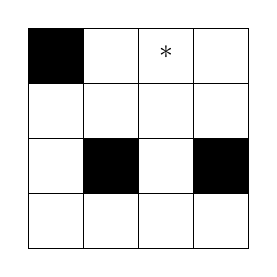
\begin{tikzpicture}[scale=0.7]
\fill[color=black] (1,1) rectangle (2,2);
\fill[color=black] (3,1) rectangle (4,2);
\fill[color=black] (0,3) rectangle (1,4);
\node at (2.5,3.5) {*};
\draw (0,0) grid (4,4);
\end{tikzpicture}
\end{center}

Әуелде * арқылы белгіленген ақ ұяшықтан
қара ұяшыққа минимум қашықтықты есептейміз.
Минимум қашықтық -- 2, яғни екі қадам солға жүріп,
қара ұяшыққа жете аламыз. Кейін ақ ұяшықты
қараға бояймыз:

\begin{center}
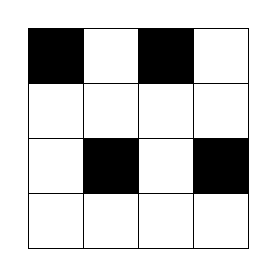
\begin{tikzpicture}[scale=0.7]
\fill[color=black] (1,1) rectangle (2,2);
\fill[color=black] (3,1) rectangle (4,2);
\fill[color=black] (0,3) rectangle (1,4);
\fill[color=black] (2,3) rectangle (3,4);
\draw (0,0) grid (4,4);
\end{tikzpicture}
\end{center}

Төмендегі екі алгоритмді қарастырайық:

\emph{1-алгоритм:} Ені бойынша іздеу (BFS) арқылы 
әр ақ ұяшық үшін ең жақын орналасқан қара ұяшықты 
анықтаймыз. Бұл $O(n)$ уақыт алады және әр ізденістен кейін
әр ақ ұяшықтан қара ұяшыққа дейінгі қашықтықты $O(1)$ уақытта
айта аламыз.

\emph{2-алгоритм:} Қараға боялған ұяшықтарды 
тізімде сақтаймыз, әр операция сайын тізімді 
өтіп шығып, соңында жаңа ұяшық қосамыз.
Операция $O(k)$ уақыт алады, мұндағы $k$ -- тізімнің өлшемі.

Операцияларды әрқайсысы $O(\sqrt n)$ операциядан
тұратын $O(\sqrt n)$ \emph{дестелерге}
бөлу арқылы жоғарыдағы екі алгоритмді біріктіреміз. 
Әр дестенің алдында біз 1-алгоритмді жүргіземіз.
Кейін дестедегі операцияларды өңдеу үшін 
2-алгоритмді қолданамыз. Дестелер арасында
2-алгоритмнің тізімін тазартып отырамыз. 
Әр операцияда қара ұяшыққа дейінгі минималды қашықтық --
1-алгоритмнен есептелген қашықтық немесе
2-алгоритмнен есептелген қашықтық болады. 

Қорытынды алгоритм $O(n \sqrt n)$ уақытта
жұмыс істейді. Біріншіден, 1-алгоритм $O(\sqrt n)$ мәрте
орындалады және әр ізденіс $O(n)$ уақыт алады.
Екіншіден, дестенің ішінде 2-алгоритмді қолданғанда,
тізім $O(\sqrt n)$ элементті қамтиды (себебі біз
дестелер арасында тізімді тазартамыз).
Демек әр операция $O(\sqrt n)$ уақыт алады. 

\section{Бүтін бөлінулер}

Кейбір квадраттық түбір алгоритмдер 
мынадай бақылауға негізделеді:
егер $n$ бүтін саны бүтін қосылғыштармен
көрсетілсе, қосылғыштардың саны 
ең көбі $O(\sqrt n)$
\emph{әртүрлі} саннан тұрады. 
Себебі қосылғыштардың саны көп болатын және
әртүрлі қосылғыштардан тұратын қосындыны 
құрау үшін ең \emph{кішкентай}
сандарды алуымыз қажет.

Егер сандарды $1,2,\ldots,k$ деп алсақ,
қорытынды қосынды \[\frac{k(k+1)}{2}.\] болады. 
Демек максималды әртүрлі қосылғыштардың саны 
-- $k = O(\sqrt n)$. Кейін бұл бақылауға
сүйеніп, 2 есептің шығару жолын талқылаймыз. 

\subsubsection{Қоржын}

Бізге қосындысы $n$ болатын бүтін салмақтар тізімі берілген.
Салмақтардың ішжиындарынан құралатын барлық
қосындыларды табуымыз керек. Мысалы, егер салмақтар $\{1,3,3\}$ болса,
төмендегідей қосындылардың болуы мүмкін:

\begin{itemize}[noitemsep]
\item $0$ (бос жиын)
\item $1$
\item $3$
\item $1+3=4$
\item $3+3=6$
\item $1+3+3=7$
\end{itemize}

Қарапайым қоржын тәсілін (7.4-тарауын қараңыз) қолдансақ,
есеп былай шығарылады: 
$\texttt{possible}(x,k)$ функциясының мәні
алғашқы $k$ салмақты пайдаланып $x$ қосындысын жинаса, 1-ге тең, ал басқа жағдайда 0-ге тең болады. Салмақтардың
қосындысы $n$ болғандықтан, ең көбі $n$ салмақ бола алады
және функцияның барлық мәндері динамикалық бағдарламалау 
арқылы $O(n^2)$ уақытта есептеледі. 

Бірақ, әртүрлі салмақтардың саны ең
көбі $O(\sqrt n)$ болатындықтан, бұл 
алгоритмді жылдамырақ жаза аламыз.
Осылайша бірдей салмақтарды топтастырып
қарастырамыз. Әр топты $O(n)$ уақытта
өңдей аламыз, демек ақырғы уақытша күрделілігі --
$O(n \sqrt n)$. 

Идеясы осы уақытқа дейін өңделген топтарды пайдаланып,
құруға болатын салмақтарды сақтайтын жиым қолдануға негізделеді. 
Жиым $n$ элементтен тұрады. Егер $k$ қосындысын құрай
алса, $k$-элемент 1-ге, ал кері жағдайда 0-ге тең. 
Салмақтардың тобын өңдеу үшін жиымды солдан 
оңға қарай өтіп, осы топ пен алдыңғы топ арқылы 
құрауға болатын жаңа салмақтарды сақтаймыз. 

\subsubsection{Жол құрылысы}

Ұзындығы $n$ болатын \texttt{s} жолы берілген
және жалпы ұзындығы $m$ болатын $D$ жолдар жиыны берілген.
$D$ жолдарының конкатенациясы арқылы \texttt{s} жолын 
қанша жолмен құрауға болатынын қарастырайық. 

Мысалы,
егер $\texttt{s}=\texttt{ABAB}$ және
$D=\{\texttt{A},\texttt{B},\texttt{AB}\}$ болса,
онда 4 жол бар:

\begin{itemize}[noitemsep]
\item $\texttt{A}+\texttt{B}+\texttt{A}+\texttt{B}$
\item $\texttt{AB}+\texttt{A}+\texttt{B}$
\item $\texttt{A}+\texttt{B}+\texttt{AB}$
\item $\texttt{AB}+\texttt{AB}$
\end{itemize}

Бұл есепті динамикалық бағдарламалау арқылы шығаруға болады:
$\texttt{count}(k)$ деп $D$-дағы жолдар арқылы 
$\texttt{s}[0 \ldots k]$ префиксін құрайтын жолдар 
санын белгілейік. Енді $\texttt{count}(n-1)$ 
есеп жауабы бола алады және бұл есепті $O(n^2)$ уақытта
префикс дарағы арқылы шығара аламыз. 

Алайда жол хеші мен $D$-да ең көбі 
$O(\sqrt m)$ әртүрлі жолдар ұзындығы болатыны туралы бақылаудың 
арқасында жылдамырақ шешуге болады. Алдымен $D$–дағы барлық
жолдардың хэштері бар $H$ жиынын құрастырамыз.
Кейін $\texttt{count}(k)$ мәнін есептеу үшін
$D$-да болуы мүмкін жол ұзындығы $p$ мәндерін қарастырамыз және
$\texttt{s}[k-p+1 \ldots k]$ хэш мәнін есептеп,
оның $H$–та бар-жоғын тексереміз. Ұзындықтары әртүрлі
жолдардың ең көп саны $O(\sqrt m)$ болғандықтан,
қорытынды уақытша күрделілігі $O(n \sqrt m)$ болады.

\section{Мо алгоритмі}

\index{Мо алгоритмі}

\key{Мо алгоритмі}\footnote{\cite{cod15}–ге сәйкес бұл алгоритм қытайлық
спорттық бағдарламалаушы Мо Таоның атымен аталған. Алайда 
бұл техника әдебиетте ертерек пайда болды \cite{ken06}.}
\emph{статикалық} (яғни сұратымдардың арасында жиым өзгермейді)
жиымда аралық сұратымдарды өңдеуді талап ететін
көптеген есептерде қолданылады. Әр сұратымда бізге 
$[a,b]$ аралығы берілген және $a$ мен $b$ аралығындағы 
жиым элементтеріне негізделген мәнді есептеу қажет. 
Статикалық жиым болғандықтан сұратымдарды кез келген
ретте өңдеуге болады. Мо алгоритмі сұратымдарды алгоритмнің жылдам болуына кепілдік беретіндей арнайы ретпен өңдейді. 

Мо алгоритмі жиымның \emph{белсенді аралығын} сақтайды
және белсенді аралыққа қатысты сұратымға әрқашан жауап береді.
Алгоритм сұратымдарды бір-бірден өңдейді және
элементтерді қосып, не өшіріп отырып, 
белсенді аралықтың шеткі нүктелерін жылжытады. 
Уақытша күрделілігі -- $O(n \sqrt n f(n))$,
мұндағы жиым $n$ элементтен тұрады, $n$ сұратым бар және
элементті қосу немесе өшіру $O(f(n))$ уақыт алады. 

Мо алгоритмінің айласы -- сұратымдарды өңдеу
реті. Жиым $k=O(\sqrt n)$ элементтен тұратын
блоктарға бөлінеді. Егер
\begin{itemize}
\item $\lfloor a_1/k \rfloor < \lfloor a_2/k \rfloor$ немесе
\item $\lfloor a_1/k \rfloor = \lfloor a_2/k \rfloor$ және $b_1 < b_2$
\end{itemize} шарты орындалса,
$[a_1,b_1]$ сұратымы
$[a_2,b_2]$ сұратымнан ертерек өңделеді.

Осылайша, сол жақ шеткі нүктесі бір блокта тұрған барлық
сұратымдар оң жақ шеткі нүктелеріне қарай сұрыпталған ретте
бірінен кейін бірі өңделеді. Осы рет бойынша алгоритм тек 
$O(n \sqrt n)$ операция орындайды. Сол жақ шеткі нүкте 
$O(n)$ рет $O(\sqrt n)$ қадамға өзгереді, ал оң жақ
шеткі нүкте $O(\sqrt n)$ рет $O(n)$ қадамға өзгереді. 
Демек алгоритм барысында екі шеткі 
нүктелер жалпылай $O(n \sqrt n)$ қадам жасайды. 

\subsubsection*{Өрнек}

Өрнек ретінде жиым бойынша бірнеше сұратым берілді делік.
Әр сұратымда қанша \emph{әртүрлі} сан бар екенін табуымыз керек. 

Мо алгоритмінде сұратымдар әрдайым бірдей сұрыпталған,
бірақ есепке қарай сұратымға жауап қалай сақталанатыны
белгілі болады. Бұл есепте \texttt{count} жиымын белгілейік.
$\texttt{count}[x]$ деп  $x$ саны белсенді аралықта қанша рет
кездесетінін көрсетеді. 

Бір сұратымнан екінші сұратымға көшкенде,
белсенді аралық өзгереді. Мысалы, белсенді
аралық төмендегідей,
\begin{center}
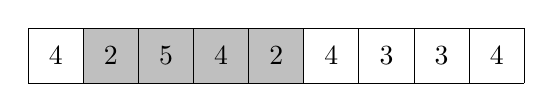
\begin{tikzpicture}[scale=0.7]
\fill[color=lightgray] (1,0) rectangle (5,1);
\draw (0,0) grid (9,1);
\node at (0.5, 0.5) {4};
\node at (1.5, 0.5) {2};
\node at (2.5, 0.5) {5};
\node at (3.5, 0.5) {4};
\node at (4.5, 0.5) {2};
\node at (5.5, 0.5) {4};
\node at (6.5, 0.5) {3};
\node at (7.5, 0.5) {3};
\node at (8.5, 0.5) {4};
\end{tikzpicture}
\end{center}
ал келесі аралық көрсетілгендей болса,
\begin{center}
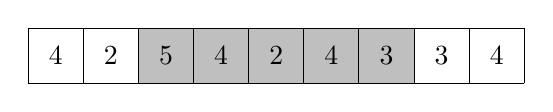
\begin{tikzpicture}[scale=0.7]
\fill[color=lightgray] (2,0) rectangle (7,1);
\draw (0,0) grid (9,1);
\node at (0.5, 0.5) {4};
\node at (1.5, 0.5) {2};
\node at (2.5, 0.5) {5};
\node at (3.5, 0.5) {4};
\node at (4.5, 0.5) {2};
\node at (5.5, 0.5) {4};
\node at (6.5, 0.5) {3};
\node at (7.5, 0.5) {3};
\node at (8.5, 0.5) {4};
\end{tikzpicture}
\end{center}
келесі үш қадам жасалу керек:
сол жақ шеткі нүкте бір қадам оңға жылжиды,
ал оң жақ шеткі нүкте екі қадам оңға жылжиды.

Әрбір қадамнан кейін \texttt{count} жиымы жаңаруы
тиіс. $x$ санын қосқаннан кейін, біз $\texttt{count}[x]$
мәнін 1-ге арттырып, кейін $\texttt{count}[x]=1$
болса, осы сұратымға байланысты жауапты 1-ге арттыруымыз қажет.
Дәл солай, $x$ санын өшіргеннен кейін, біз $\texttt{count}[x]$
мәнін 1-ге азайтып, ал одан кейін $\texttt{count}[x]=0$ болса,
осы сұратымға байланысты жауапты 1-ге азайтуымыз қажет. 

Бұл есепте әрбір қадамды орындау үшін $O(1)$ уақыт керек.
Демек алгоритмнің қорытынды уақытша күрделілігі 
-- $O(n \sqrt n)$.